\documentclass[a4paper,11pt,onecolumn,oneside]{article}
\usepackage[T1]{fontenc} 
\usepackage[utf8]{inputenc} 
\usepackage{graphicx}
\usepackage{hyperref} % para autoref
\usepackage{url}
\usepackage[printonlyused]{acronym}
\usepackage{xcolor}
\usepackage{lmodern}
\usepackage{textcomp}
\usepackage{imakeidx}
\makeindex


\begin{document}
%%
% Definições
%
\def\titulo{Trabalho de Aprofundamento 2}
\def\data{09 de maio de 2020}
\def\autores{Mariana Silva, Marta Oliveira}
\def\autorescontactos{(98392) marianabarbara@ua.pt, (97613) marta.alex@ua.pt}
\def\versao{VERSAO 1}
\def\departamento{Departamento de Eletrónica,Telecomunicações e Informática }
\def\empresa{Universidade de Aveiro}
\def\logotipo{ua.pdf}

%
%%%%%% CAPA %%%%%%
%
\begin{titlepage}

\begin{center}
%
\vspace*{50mm}
%
{\Huge \titulo}\\ 
%
\vspace{10mm}
%
{\Large \empresa}\\
%
\vspace{10mm}
%
{\LARGE \autores}\\ 
%
\vspace{30mm}
%
\begin{figure}[h]
\center
\includegraphics{\logotipo}
\end{figure}
%
\vspace{30mm}
\end{center}
%
\begin{flushright}
\versao
\end{flushright}
\end{titlepage}

%%  Página de Título %%
\title{%
{\Huge\textbf{\titulo}}\\
\vspace{10mm}
{\Large \departamento\\ \empresa}
}
%
\author{%
    \autores \\
    \autorescontactos
}
%
\date{\data}
%
\maketitle

\pagenumbering{roman}

%%%%%%%%%%%%%%%%%%%%%%%%%%%%%%%
\clearpage
\pagenumbering{arabic}

\newpage

{\center \tableofcontents}     
{\center \listoffigures}  

\newpage

{\center \section{Introdução}}
\paragraph{ }
O tema proposto deste trabalho consiste em seriar, de forma aleatória, n clientes. De forma a que este serviço seja gerado de forma isenta, as aplicações cliente irão usar interfaces abertas.
\paragraph{ }
Resumidamente:
\paragraph{ }
Iremos ter uma interface/aplicação cliente-servidor.
\paragraph{ }
Neste código, iremos utilizar os fundamentos da \ac{api} de Sockets.
\paragraph{ }
\textbf{Aplicação Cliente:}

\renewcommand{\theenumi}{\arabic{enumi}}
\begin{enumerate}
\item Criar o socket (função socket);
\item A seguir, criar uma função connect para conectar com o servidor;
\item Enviar/Receber dados enquanto existem dados para enviar/receber;
\item Fechar o socket. 
\end{enumerate}

\paragraph{ }
\textbf{Aplicação Servidor:}
\renewcommand{\theenumi}{\arabic{enumi}}
\begin{enumerate}
\item Criar o socket (função socket);
\item Inserir um endereço \ac{ip} e uma porta no socket (função bind);
\item A função accept serve para aceitar uma nova conexão;
\item Fechar o socket.
\item Podem ser usadas várias conexões, por isso o passo 3 pode ser repetido;
\end{enumerate}

Os passos do servidor são feitos usando o \ac{tcp} 
\paragraph{ }
Para além disso, neste relatório, iremos explicar a implementação não só do código como também do algoritmo, apresentar testes que comprovam o seu funcionamento e analisar os resultados obtidos.
\paragraph{ } 
Este Trabalho de Aprofundamento foi criado no code.ua.pt com o nome labi2020-ap2-g45 (\url{https://code.ua.pt/projects/labi2020-ap2-g45}).

\newpage

{\center \section{Código}}

\paragraph{ }
Começámos por executar a simulação da aplicação cliente servidor para confirmar se tudo funcionava como previsto (testes iniciais).

\subsection{Terminal}
\paragraph{ }
Quando ficheiro do server é iniciado, o terminal não mostra nenhuma mensagem como seria esperado.

\begin{figure} [h]
\center
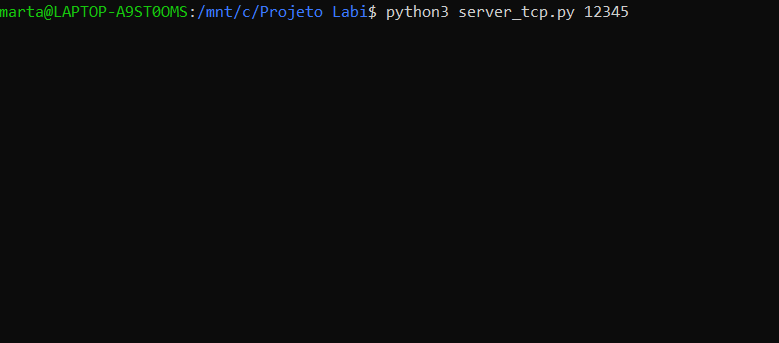
\includegraphics[width=350px]{terminal1.png}
\caption{Terminal 1}
\label{terminal1}
\end{figure}

\paragraph{ }

Ao iniciarmos o segundo terminal e ao executar o ficheiro do cliente iremos encontrar o seguinte “menu” no terminal.

\begin{figure} [h]
\center
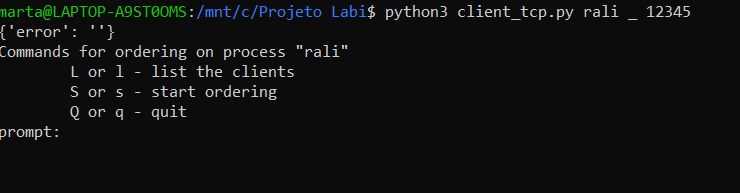
\includegraphics[width=350px]{terminalcliente.png}
\caption{Terminal 2}
\label{terminal2}
\end{figure}

\paragraph{ }
Como não temos participantes temos que iniciar um terceiro terminal e colocar 10 participantes (usando a Shell script- run\textunderscore tcp).

\begin{figure} [h]
\center
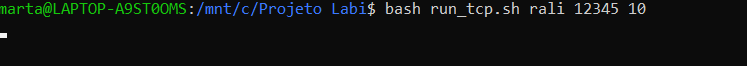
\includegraphics[width=350px]{terminalsemclientes.png}
\caption{Terminal 3}
\label{terminal3}
\end{figure}

\newpage
\paragraph{ }
Logo após lançar este comando, o terminal 1 aparece da seguinte forma (uma mensagem de pedido a cada cliente)


\begin{figure} [h]
\center
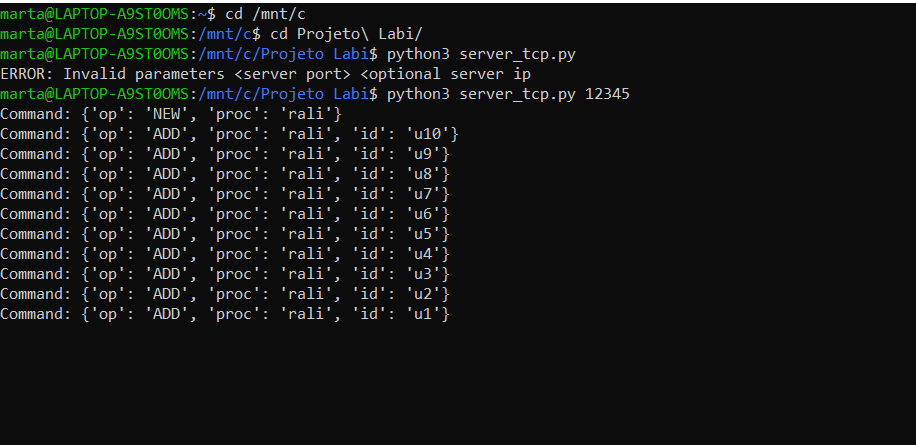
\includegraphics[width=350px]{terminal1seguinte}
\caption{Terminal 1 após comando}
\label{terminal1seguinte}
\end{figure}


\paragraph{ }
Para além disso, também nos apercebemos que se os dados forem mal inseridos no terminal irá aparecer uma mensagem de erro onde pede a forma correta de inserir as “informações”.

\paragraph{ }
Ao voltarmos ao terminal 2 e ao carregarmos no L (para listarmos clientes), o programa já nos irá lançar os 10 clientes.

\begin{figure} [h]
\center
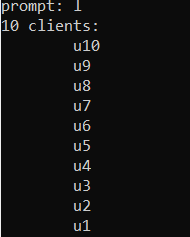
\includegraphics[height=130px]{terminal2seguinte.png}
\caption{Terminal 2 após comando}
\label{terminal2seguinte}
\end{figure}

\newpage
\subsection{Explicação do código b64.py}

\begin{figure} [h]
\center
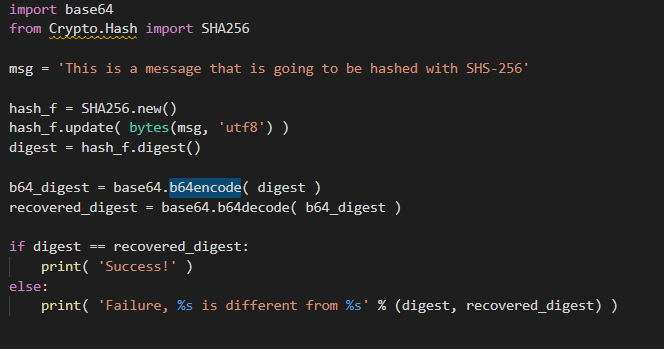
\includegraphics[width=350px]{base64.png}
\caption{Código base64}
\label{base64}
\end{figure}

\paragraph{ }
Neste código, o SHA-2 irá funcionar com funções hash.
\paragraph{ }
A função hash basicamente, resume dados. Vai buscar elementos/dados de qualquer tamanho e transforma-os em dados de comprimentos fixos.
\paragraph{ }
Sendo assim, o resultado da função hash irá ser diferente do valor original.
\paragraph{ }
Com este método, não iremos conseguir descobrir o valor original (de entrada). Sendo assim, este método irá ser bastante importante pois, a partir do mesmo é possível garantir a segurança das chaves dos clientes.
\paragraph{ }
Comparando o hash que saiu (recovered\textunderscore digest) ao valor de hash inicial/inserido (digest), a pessoa pode aperceber-se da segurança dos dados, porque irá obter resultados idênticos.




\newpage
\subsection{Explicação do código cifradecifra.py}

\begin{figure} [h]
\center
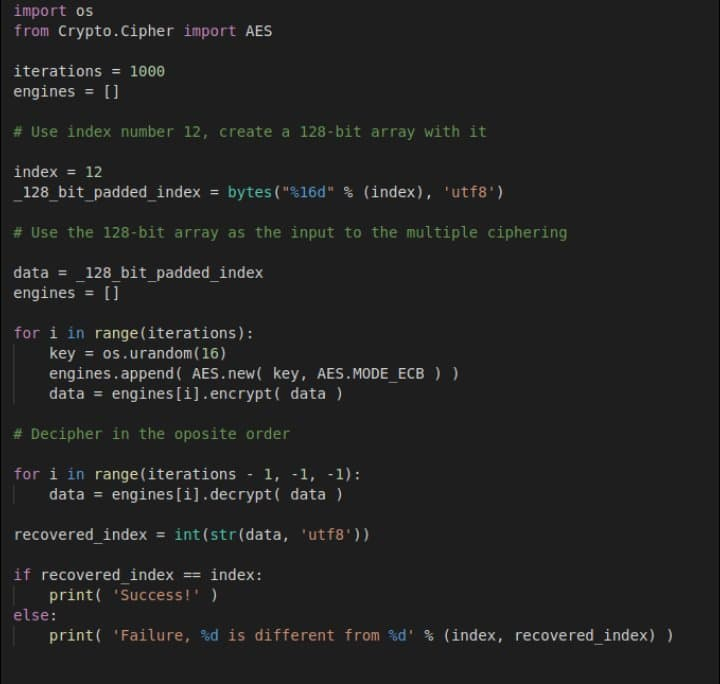
\includegraphics[width=350px]{cifradecifra.png}
\caption{Código cifra/decifra}
\label{cifra/decifra}
\end{figure}
\paragraph{ }
De forma a manter a segurança das chaves, iremos usar criptografia.
\paragraph{ }
Para tal, iremos buscar as chaves no ciclo for e o método .urandom irá servir para gerar uma sequência de bytes (neste caso, 16).
\paragraph{ }
A variável criptografada (data) agora terá o valor da mensagem criptografada em bytes.
\paragraph{ }
Para descriptografar a mensagem iremos precisar da mesma chave e da mensagem criptografada (que ainda se encontra em bytes - data).
\paragraph{ }
A variavel descriptografada  deverá ter o mesmo valor da mensagem original e por isso é que está feito o if (por questões de segurança).

\newpage
\subsection{Explicação do código tcp}

\begin{figure} [h]
\center
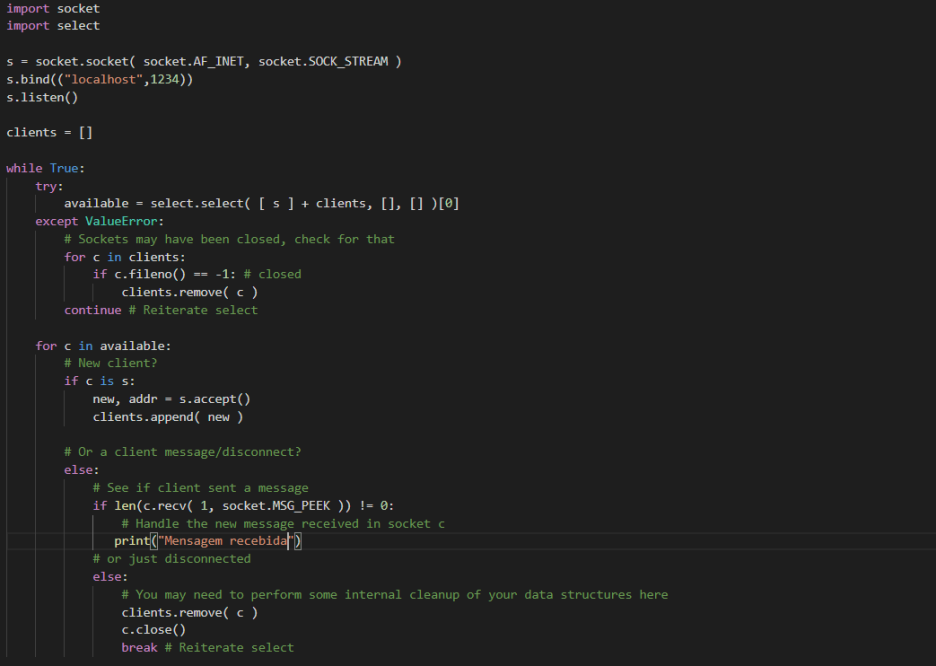
\includegraphics[width=350px]{tcp.png}
\caption{Código tcp}
\label{tcp}
\end{figure}

\paragraph{ }
Em primeiro, é necessário criar um socket.
\paragraph{ }
O servidor irá ter um método bind() que o liga a um \ac{ip} e portas para que ele possa "ouvir" os pedidos recebidos. 
\paragraph{ }
O server também terá um método listen() que coloca o servidor no modo de "escuta". Isto permite que o servidor vá receber/ouvir os pedidos de entrada. 
\paragraph{ }
Por último, o servidor possui um método accept() e close(). O método accept aceita e inicia uma conexão com o cliente e o método close fecha a conexão com o cliente.
\paragraph{ }
Se o cliente estiver "disponível" (available) iremos selecioná-lo e verificar se é novo ou se já enviou alguma mensagem (poderá ser um pedido para desconectar).


\newpage
\subsection{Explicação do Algoritmo do server\textunderscore tcp}


\begin{figure} [h]
\center
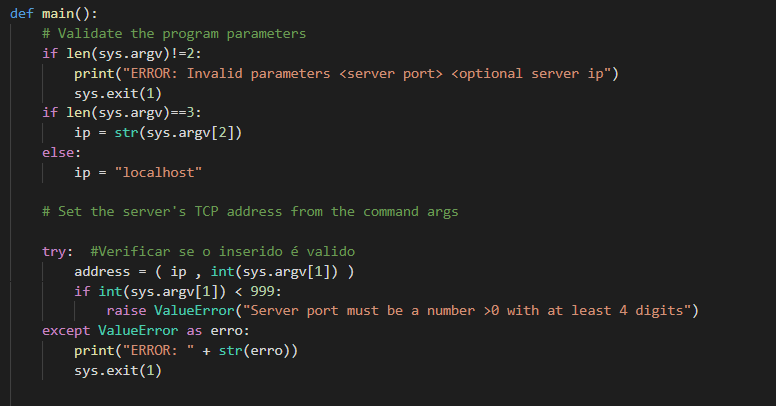
\includegraphics[width=350px]{def_main_do_server.png}
\caption{Função main do server}
\label{main server}
\end{figure}

\paragraph{ }
No máximo, pode-se inserir como argumentos o port do server e, opcionalmente, o server ip.
Se não for optado por se dizer o server ip então será assumido como “localhost”.

\begin{figure} [h]
\center
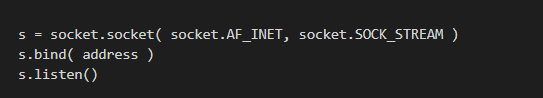
\includegraphics[width=350px]{AFINET.png}
\caption{Sockets}
\label{Sockets}
\end{figure}

\paragraph{ }
O servidor que irá receber as mensagens do client.sockets irá enviar dados através da rede. Assim, o socket irá receber a conexão onde passam dois argumentos.
\paragraph{ }
\textbf{AF\textunderscore INET} refere-ae à família de endereços IPv4 (figura \ref{Sockets}).
\paragraph{ }
\textbf{SOCK\textunderscore STREAM} significa que é um socket \ac{tcp} (figura \ref{Sockets}).

\begin{figure} [h]
\center
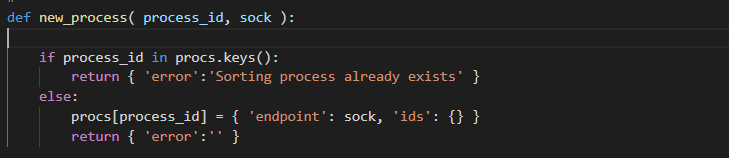
\includegraphics[width=350px]{entradadecliente.png}
\caption{Função new\textunderscore process}
\label{process}
\end{figure}

\paragraph{ }
O código apresentado na figura \ref{process} irá iniciar um novo processo. Irá verificar se o cliente é ou não repetido, ou seja, irá verificar se já fez ou não um processo e, por isso, verificar se já tem uma "chave" associada, ou não.

\begin{figure} [h]
\center
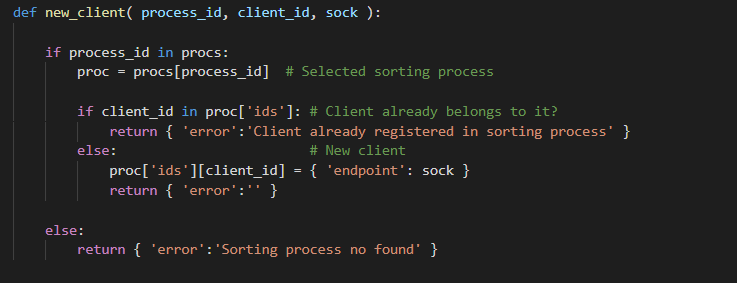
\includegraphics[width=350px]{funcaonewcliente.png}
\caption{Função new\textunderscore client}
\label{client}
\end{figure}

\paragraph{ }
A função new\textunderscore client serve para incluir um novo cliente no programa.
\paragraph{ }
No caso de o cliente já tiver realizado a sua "candidatura", o programa irá fazer o retorno de uma mensagem de erro a avisar que já está registado \textbf{(if process id)}.
\paragraph{ }
Se não estiver registado, irá ser usado um socket para receber as informações (os argumentos que entram na função são: \textbf{process\textunderscore id} e \textbf{client\textunderscore id}).

\begin{figure} [h]
\center
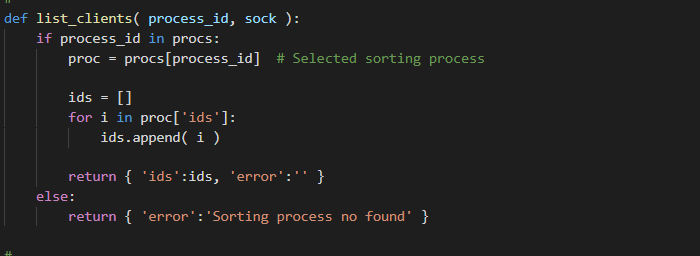
\includegraphics[width=350px]{funcaolistclients.png}
\caption{Função list\textunderscore clients}
\label{list}
\end{figure}

\paragraph{ }
Na função list \textunderscore clients, tal como o nome indica, iremos listar os clientes que já existem.
\paragraph{ }
Isso é possível, uma vez que ao usar os process \textunderscore id dos clientes, iremos realizar um ciclo \textbf{for} usando todos os ids que existem e fazendo a impressão (print) dos mesmos.

\begin{figure} [h]
\center
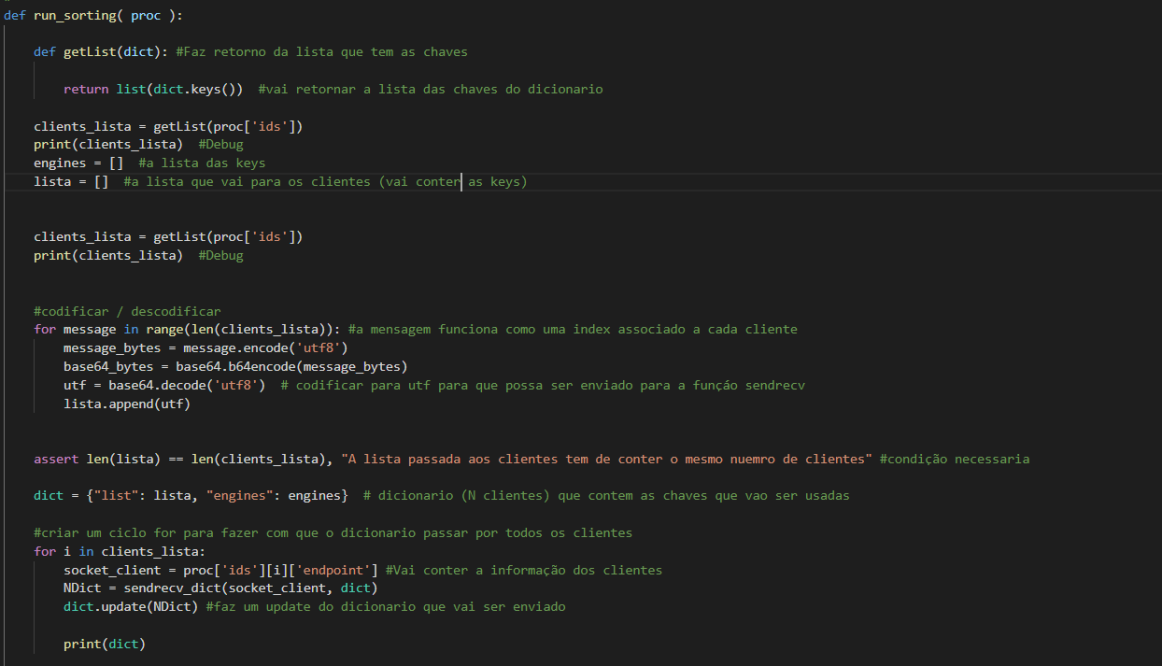
\includegraphics[width=350px]{def_run_sorting.png}
\caption{Função run\textunderscore sorting}
\label{sorting}
\end{figure}

\paragraph{ }
Esta função serve para o processo de ordenação. Em primeiro, fazemos uma lista que irá buscar as chaves contidas no dicionário (função keys()).
\paragraph{ }
Depois fazemos um ciclo for (o int message funciona como um índice de valores associado a cada cliente) para fazer o processo de descodificação de forma a que a informação possa ser enviada para a função sendrecv. 
\paragraph{ }
Fazemos um “assert” para verificar se não existe nenhuma incoerência em relação ao número de clientes.
\paragraph{ }
Quando verificado, o dicionário irá conter a lista e as chaves que irão ser usadas pelos clientes.
\paragraph{ }
A seguir, o dicionário irá passar pelos clientes para obter (recv) as informações/address dos mesmos. Consequentemente, irá atualizar o dicionário anterior (o que continha a lista e as chaves).

\newpage

\subsection{Explicação do Algoritmo do client\textunderscore tcp}

\begin{figure} [h]
\center
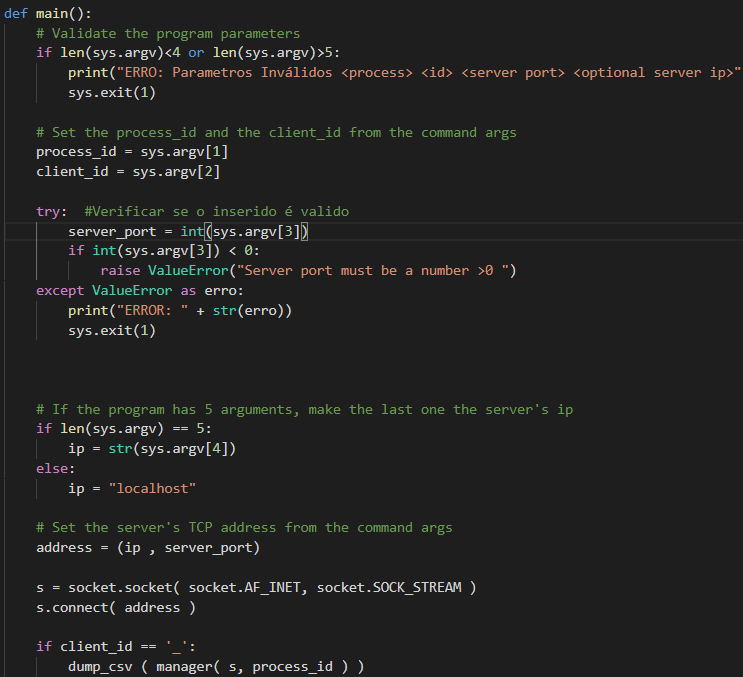
\includegraphics[width=350px]{defmaindoclient2}
\caption{Função main}
\label{main}
\end{figure}

\paragraph{ }
O \textbf{sys.Argv} contém os argumentos escritos no terminal. Os argumentos começam a contar a partir do 0.
\paragraph{ }
O \textbf{process id} é o segundo argumento que é passado no terminal (sendo o primeiro rali/corrida, por exemplo) logo o process\textunderscore id é sys.argv[1] (o identificador especial definido é o “\textunderscore”).
\paragraph{ }
O \textbf{cliente id} é o terceiro argumento que passamos no terminal (logo args[2]).
\paragraph{ }
O quarto argumento (agrs[3])passado no terminal  especifica \textbf{o porto do servidor} (\ac{tcp}).
\paragraph{ }
Faz-se um \textbf{if} no caso do cliente optar por colocar o \textbf{endereço IPv4}  (que, neste caso, \underline{é opcional}) e sendo assim passam a existir 5 argumentos sendo o último de todos eles o ip do servidor. Se não existir esta especificação, o programa assume que o cliente esteja a usar um servidor na mesma maquina onde se encontra o cliente, ou seja, \textbf{localhost}.
\paragraph{ }
Por estas razões o comprimento (len) dos argumentos só podem variar entre 4 e 5. Se forem inseridos argumentos incorretos irá aparecer uma mensagem de erro como é demonstrado na imagem.
\paragraph{ }
O \ac{tcp} deverá ser um valor inteiro positivo por isso realizámos um \textbf{Try/except} no caso do valor inserido ser inferior a 0.

\begin{figure} [h]
\center
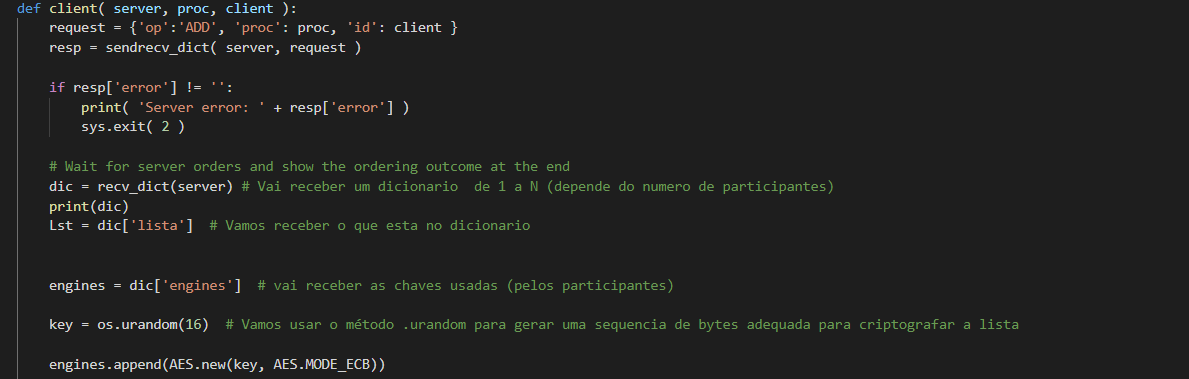
\includegraphics[width=350px]{def_client_1.png}
\caption{Função Client}
\label{função client 1}
\end{figure}

\begin{figure} [h]
\center
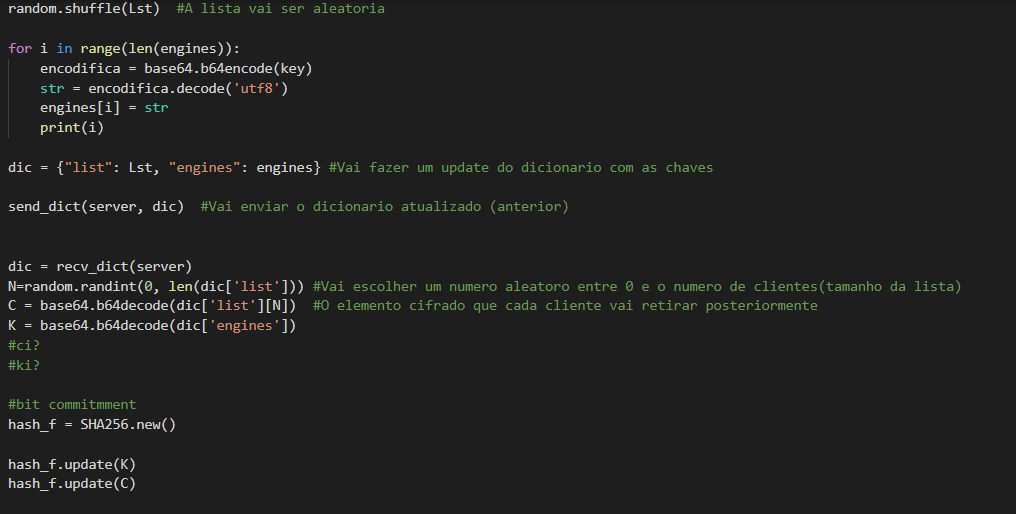
\includegraphics[width=350px]{def_client_2.png}
\caption{Continuação da Função Client}
\label{função client 2}
\end{figure}

\paragraph{ }
Nesta função, pegamos nas informações contidas no dicionário(que são recebidas do server) e descodificamo-las (tanto a chave como as listas dos clientes - N clientes).
\paragraph{ }
A lista dos clientes terá que ser aleatória, por isso fazemos o random shuffle.
\paragraph{ }
Depois de feito um update do dicionário (decifrado + lista aleatória) voltamos a enviar o dicionário para o server.
\paragraph{ }
De seguida, escolhemos um número aleatório (N) de forma a escolher um cliente qualquer (de forma isenta) para escolher a sua chave.
\paragraph{ }
Cada cliente, irá escolher um elemento cifrado (C).
\paragraph{ }
De seguida, iremos enviar a chave simétrica (K) e o elemento cifrado (C) à função hash para essas informações serem guardadas de forma segura.
\paragraph{ }
Passando ao código seguinte.


\begin{figure} [h]
\center
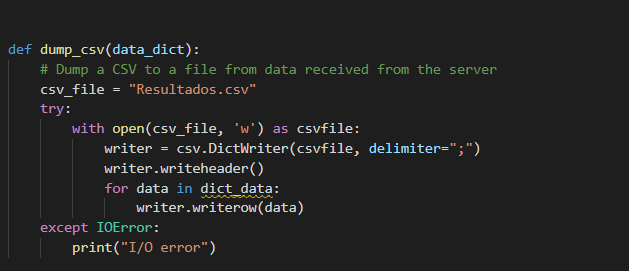
\includegraphics[width=350px]{dictwriter.png}
\caption{Função dump\textunderscore csv}
\label{dump}
\end{figure}

\paragraph{ }
Esta função serve para descarregar um csv para um ficheiro, a partir dos dados recebidos pelo servidor.
\paragraph{ }
O método dict writer está contido no módulo csv. Este facto requer o nome do ficheiro csv (que está guardado como "resultados").
\paragraph{ }
O código writeheader() grava a primeira linha no arquivo csv como nomes de campo. Consequentemente, o loop irá gravar cada linha.
\paragraph{ }
Desta forma, iremos aceder aos valores do csv.

\newpage
{\center \section{Análise dos Resultados Obtidos}}

\paragraph{ }
Não foi possível a completa análise dos resultados obtidos, uma vez que o trabalho não foi concluído na sua totalidade.


\newpage

{\center \section{Contribuição dos Autores}}
\paragraph{ }
Para a realização deste trabalho de aprofundamento, a MO desenvolveu o código na sua maioria, fazendo a respetiva pesquisa, recolhendo o maior número de elementos que contribuíssem para o desenrolar do trabalho. A MS trabalhou na estrutura e apresentação do relatório, com a implementação de textos explicativos do código e respetivos exemplos nas imagens apresentadas acerca de cada tópico. 
\paragraph{ }
Assim, cada um dos intervenientes contribuiu em igual percentagem (50\%) para os objetivos propostos neste trabalho.

\newpage
\center \begin{thebibliography} {9}
\bibitem{latexcompanion}
\url{https://stackabuse.com/encoding-and-decoding-base64-strings-in-python/}
\bibitem{latexcompanion}
\url{https://docs.python.org/3/howto/unicode.html#converting-between-file-encodings}
\bibitem{latexcompanion}
\url{https://wiki.python.org.br/SocketBasico}
\bibitem{latexcompanion}
\url{http://excript.com/python/depuracao-pycharm-python.html}
\bibitem{latexcompanion}
\url{https://www.geeksforgeeks.org/python-hash-method/}
\bibitem{latexcompanion}
\url{http://www.macoratti.net/vbn_cah1.htm}
\bibitem{latexcompanion}
\url{https://pythonhelp.wordpress.com/tag/hash/}

\end{thebibliography}

\newpage

{\huge \textbf{Acrónimos} \centering }

\begin{acronym}
\acro{api}[API]{Interface de Programação de Aplicações}
\acro{ip}[IP]{Protocolo da Internet}
\acro{tcp}[TCP]{Protocolo de Controlo de Transmissão}
\end{acronym}

\end{document}

